\section{Diagnóstico do estágio atual}

\subsection{Fase da startup}

Entre as fases indicadas na orientação (ideação, validação, tração e escala), o PetCuida está na transição entre ideação e validação. Há produto demonstrável e sinais qualitativos, mas não há usuários ativos, receita nem parceiros formalizados nas fontes analisadas. O relatório de usabilidade registra limites que precisam ficar explícitos: o mapa era esquemático, o login Google estava simulado e parte dos participantes não compreendeu de imediato os créditos e o QR Code [3].

\begin{table}[H]
\centering\small
\caption{Situação observada e proposta a validar.}
\begin{tabularx}{\textwidth}{P{2.6cm}YY}
\toprule
\textbf{Dimensão} & \textbf{Base observada} & \textbf{Proposta a validar} \\
\midrule
Produto & Protótipo com perfil do pet, calendário, triagem e rede demonstrativa. & Piloto controlado com fluxos revistos e tarefas concluídas sem ajuda. \\
Mercado & Cinco sessões qualitativas e contexto setorial amplo. & Demanda local, frequência de uso e necessidades de clínicas e tutores. \\
Receita & Sem faturamento nem preço validado. & Planos para parceiros, intermediação e patrocínio, sem pressupor adesão. \\
Parcerias & Sem contratos ou clínicas formalmente parceiras. & Interesse de organizações locais em participar de um piloto. \\
\bottomrule
\end{tabularx}
\end{table}

\begin{figure}[H]
\centering
\begin{minipage}[t]{0.29\textwidth}\centering
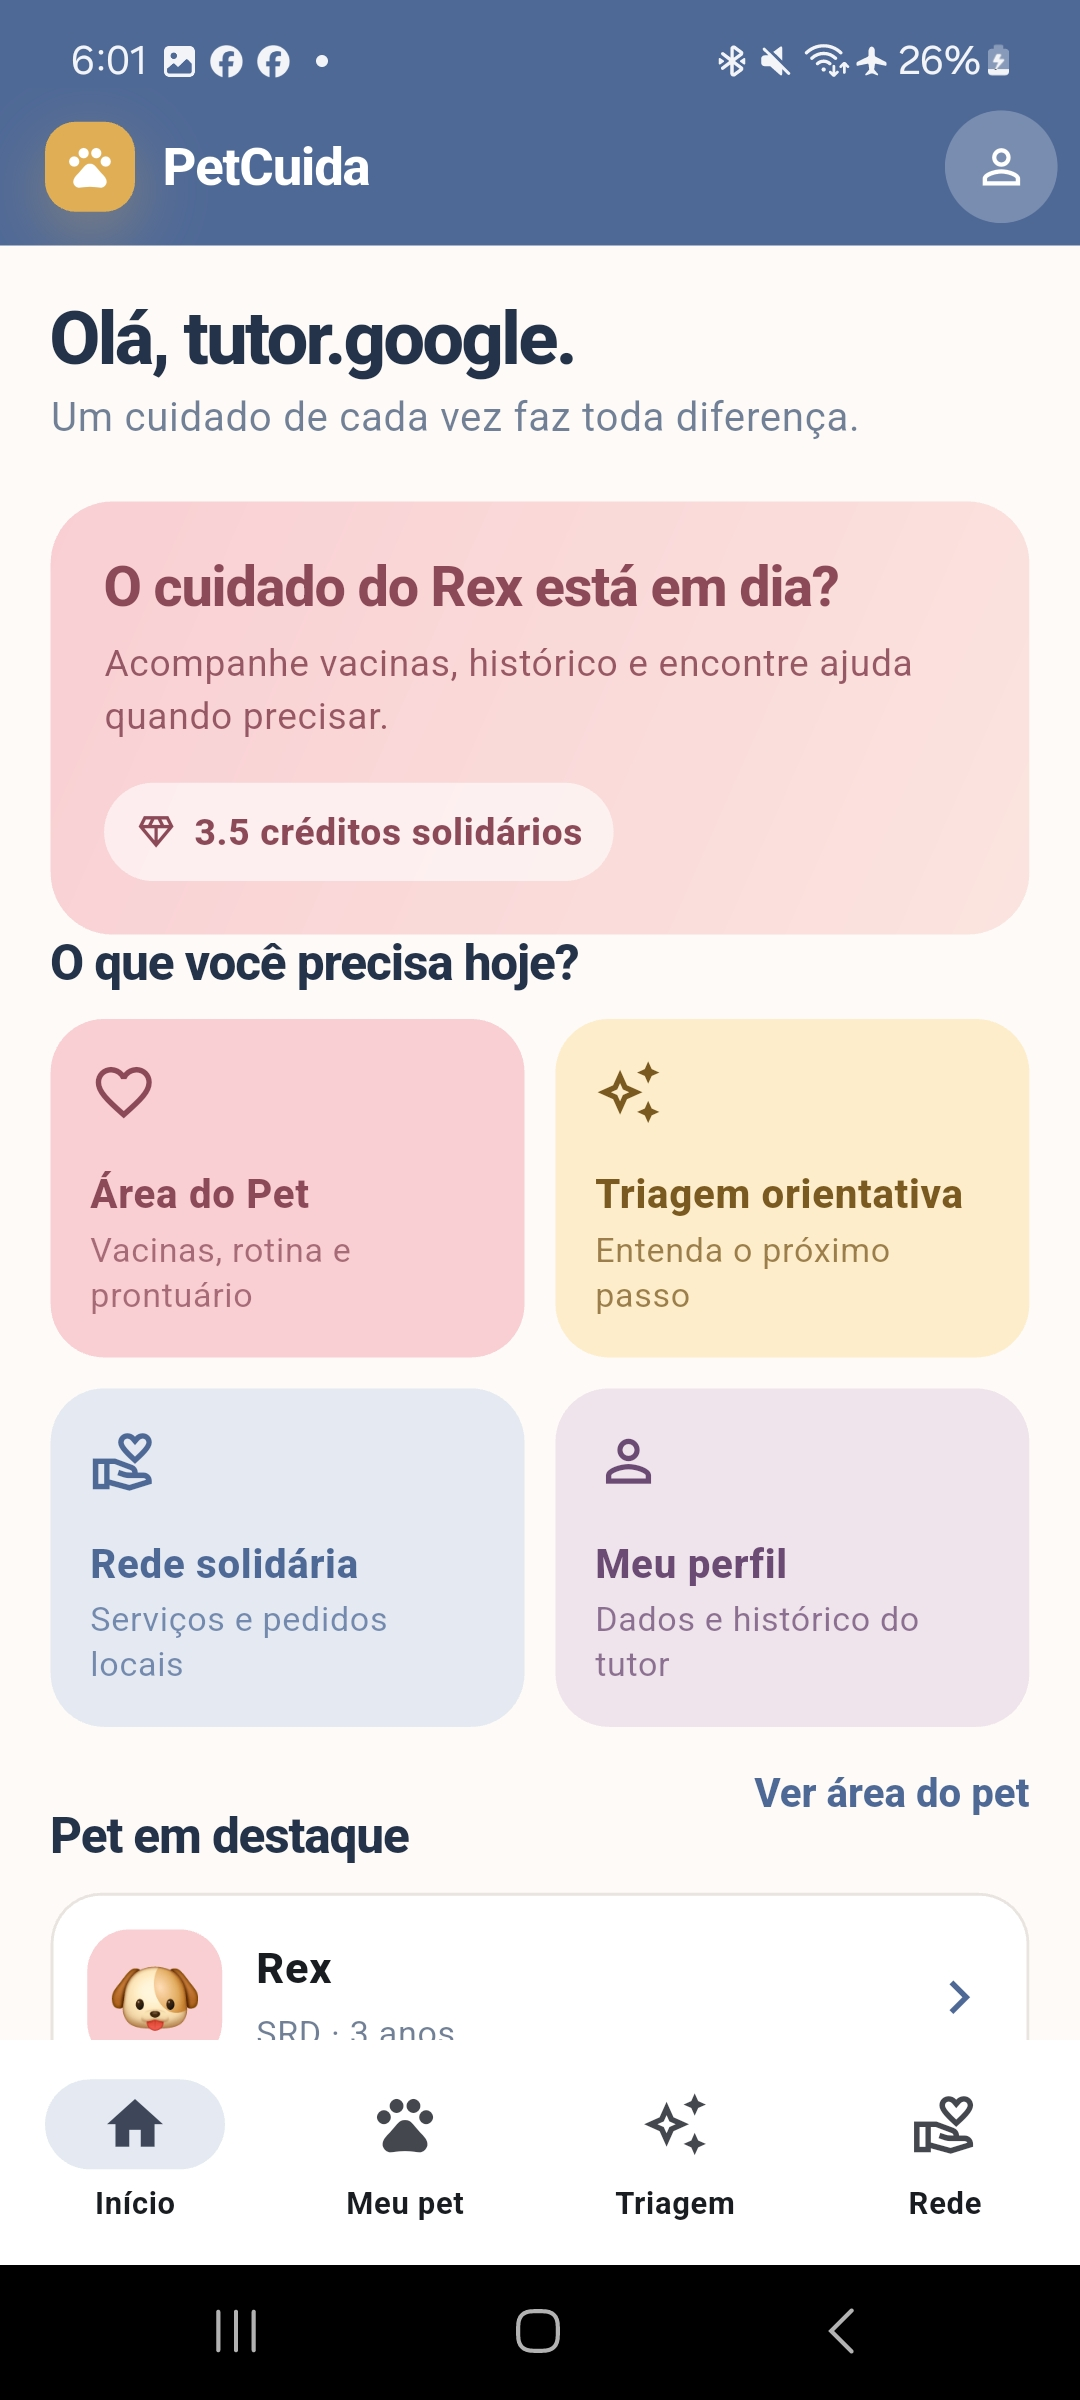
\includegraphics[height=4.5cm,keepaspectratio]{assets/tela_inicial.jpg}\\{\small Tela inicial}
\end{minipage}\hfill
\begin{minipage}[t]{0.29\textwidth}\centering
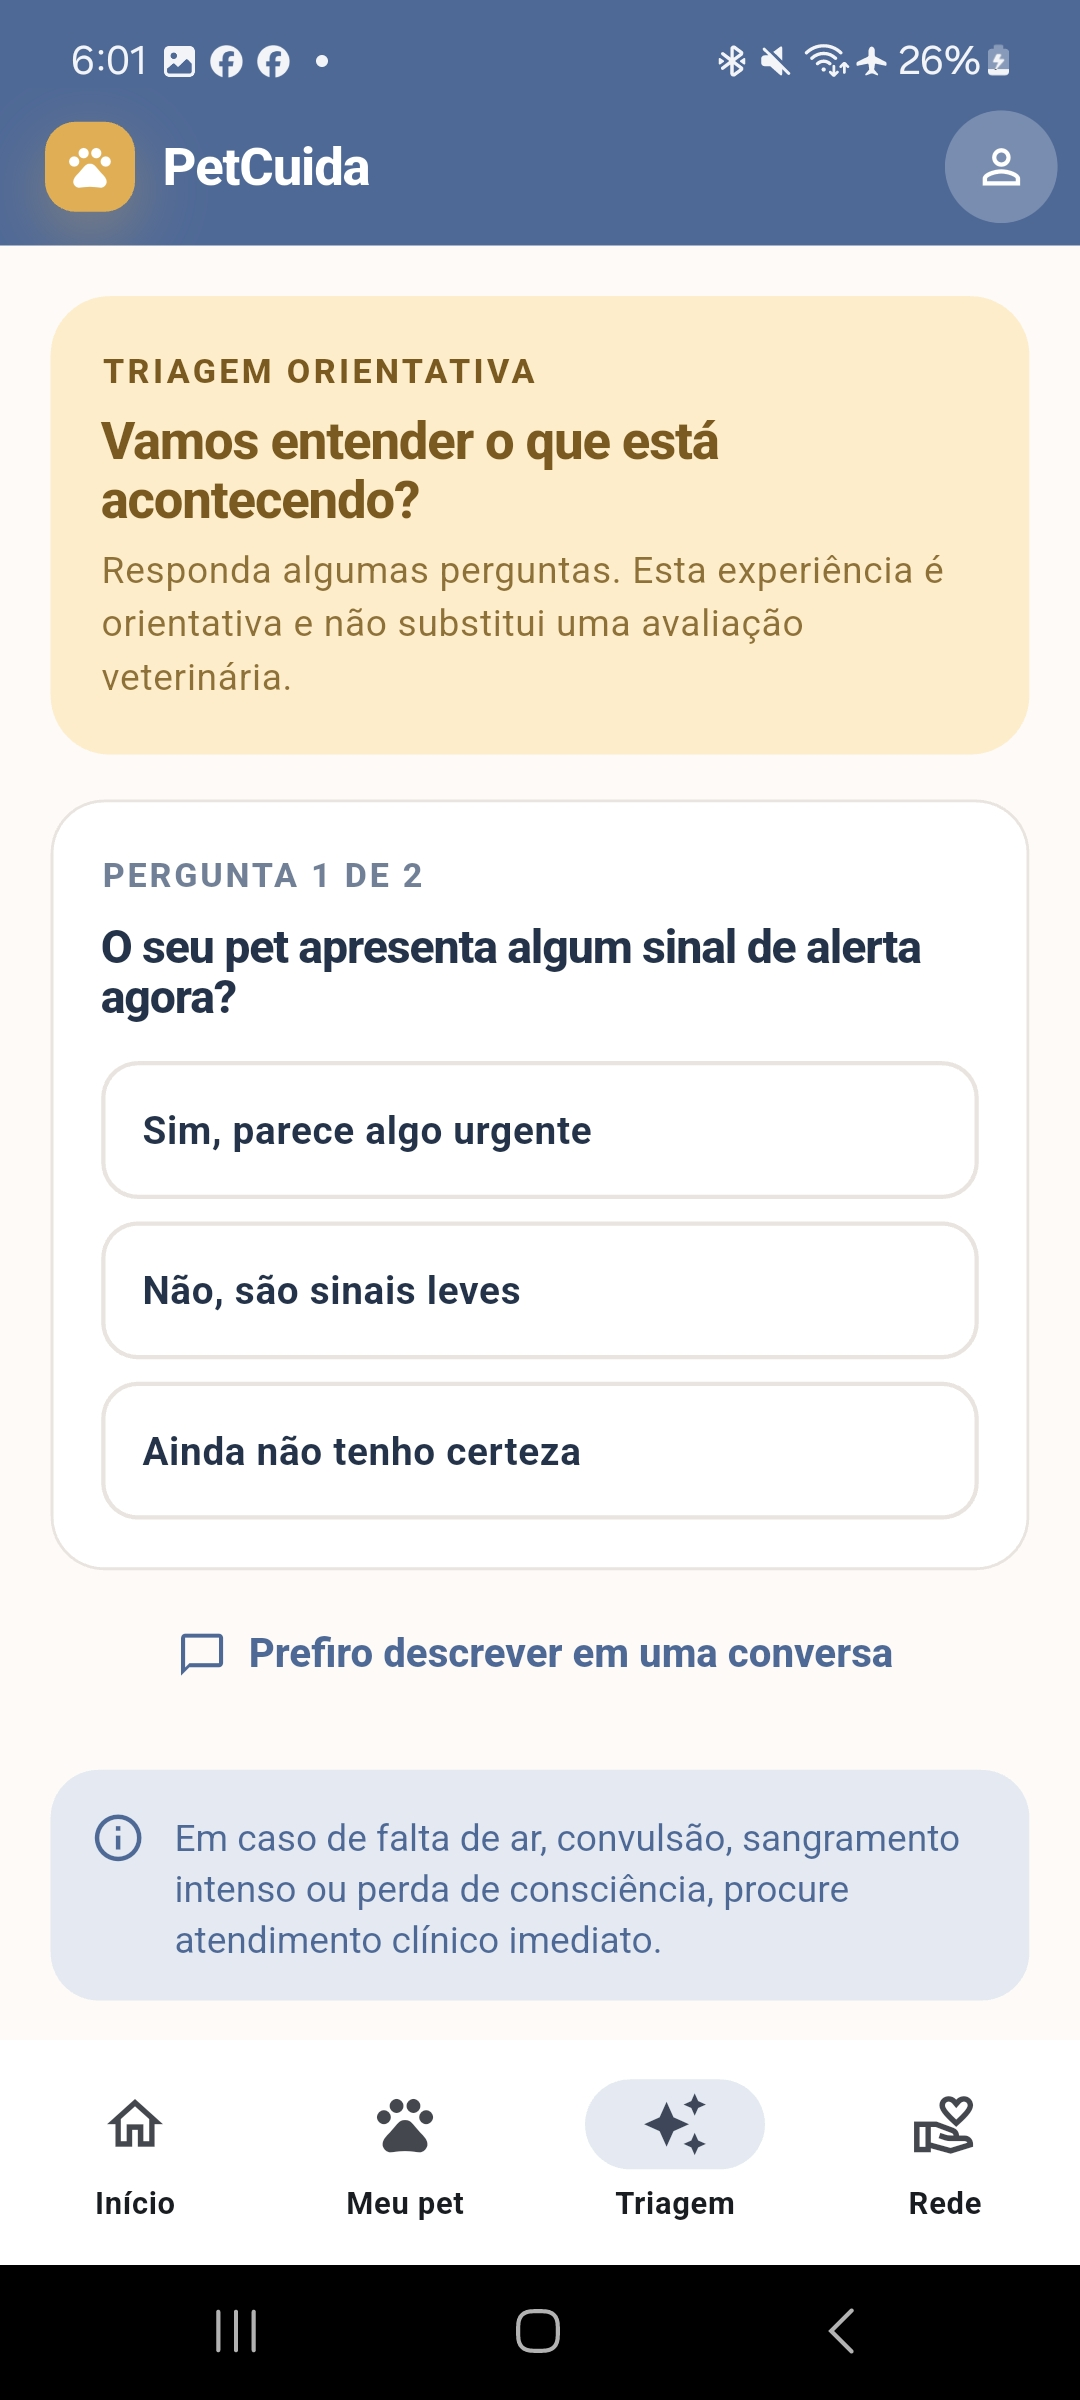
\includegraphics[height=4.5cm,keepaspectratio]{assets/tela_triagem.jpg}\\{\small Triagem orientativa}
\end{minipage}\hfill
\begin{minipage}[t]{0.29\textwidth}\centering
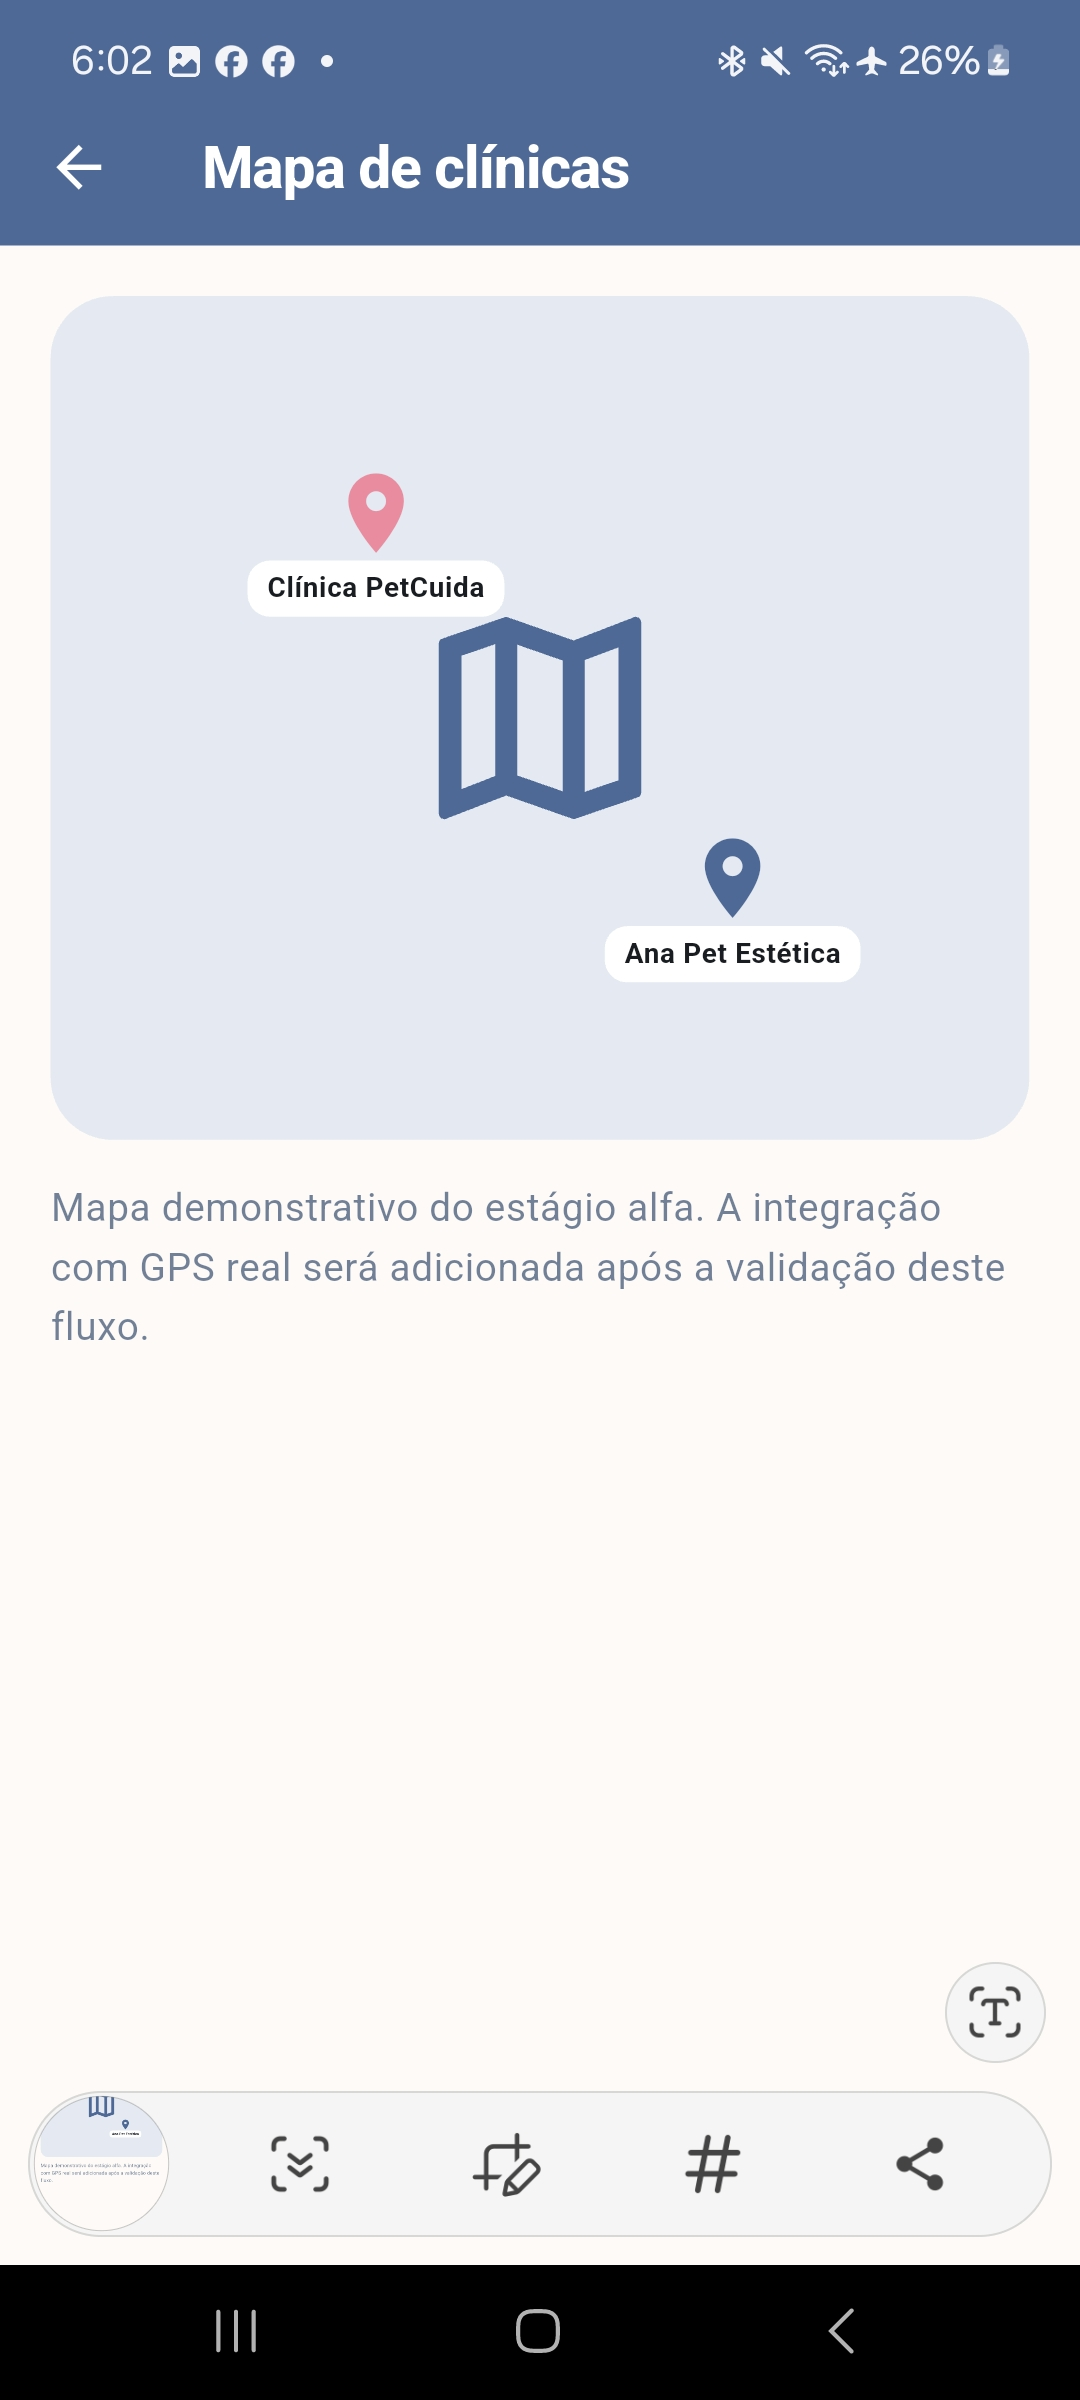
\includegraphics[height=4.5cm,keepaspectratio]{assets/tela_mapa.jpg}\\{\small Mapa demonstrativo}
\end{minipage}
\caption{Capturas do protótipo PetCuida Alpha 3i. O mapa é ilustrativo. Fonte: repositório do projeto [2, 3].}
\end{figure}

\subsection{Evidência inicial e seus limites}

As cinco sessões registraram percepção favorável de facilidade de uso, da triagem e da rede solidária diante de barreiras como custo, transporte e acesso à castração [3]. Estudos clássicos de usabilidade indicam que cerca de cinco participantes revelam boa parte dos problemas de interface [17], mas não medem adoção. A amostra foi pequena, a navegação foi conduzida pelos entrevistadores e não se aplicou escala padronizada como a SUS [18]. São sinais exploratórios, não tração.

\subsection{Contexto setorial}

Segundo a ABEMPET, o setor pet brasileiro faturou R\$ 77,96 bilhões em 2025 (+3,45\%), com serviços veterinários em torno de 10,5\% do total [19]. A população pet foi estimada em 164,7 milhões de animais em 2024 [20, 21], e a imprensa noticiou projeção de R\$ 81 bilhões para 2026 [22]. Na literatura, custo, acessibilidade, comunicação e falta de informação aparecem como as principais barreiras ao cuidado veterinário em comunidades vulneráveis [23, 24]. Esses dados mostram relevância do problema, mas não medem o mercado alcançável pelo PetCuida.

\subsection{Principais desafios}

\begin{itemize}
\item \textbf{Clareza da experiência:} créditos e QR Code não foram compreendidos por parte dos participantes [3].
\item \textbf{Uso autônomo não testado:} a navegação foi conduzida pelos entrevistadores.
\item \textbf{Oferta local:} sem clínicas e ONGs dispostas a receber encaminhamentos, a rede não entrega valor [10].
\item \textbf{Economia do serviço:} não há estimativa confiável de custos de suporte, pagamento e operação.
\item \textbf{Limites clínicos e de dados:} a triagem é orientativa [25] e o uso de dados exige conformidade com a LGPD [26].
\end{itemize}
